\section{dg::Hypertexture Class Reference}
\label{classdg_1_1Hypertexture}\index{dg::Hypertexture@{dg::Hypertexture}}
{\tt \#include $<$Hypertexture.h$>$}

Collaboration diagram for dg::Hypertexture:\begin{figure}[H]
\begin{center}
\leavevmode
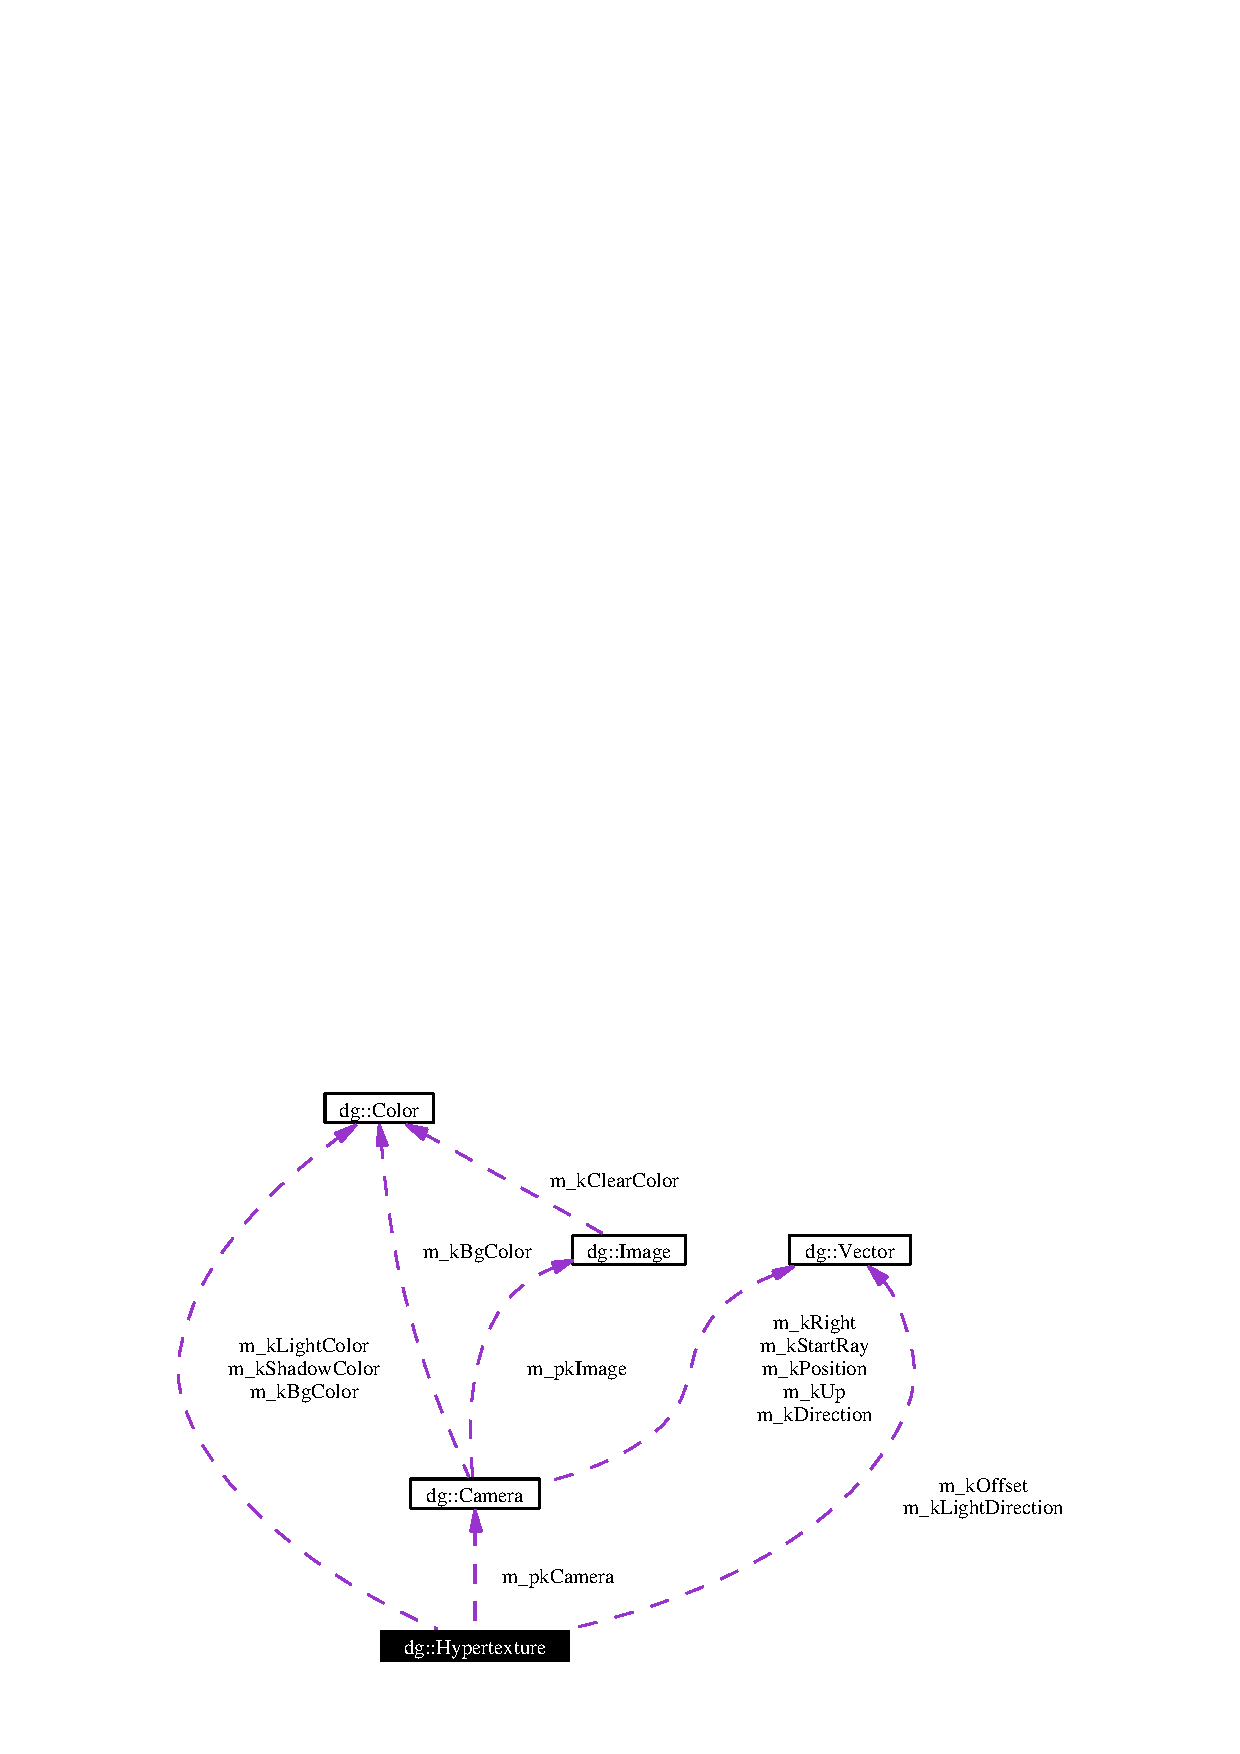
\includegraphics[width=274pt]{classdg_1_1Hypertexture__coll__graph}
\end{center}
\end{figure}
\subsection*{Public Types}
\begin{CompactItemize}
\item 
typedef {\bf Real}($\ast$ {\bf Density\-Fn} )({\bf Real} f\-X, {\bf Real} f\-Y, {\bf Real} f\-Z)
\item 
typedef {\bf Real}($\ast$ {\bf Filtered\-Density\-Fn} )({\bf Real} f\-X, {\bf Real} f\-Y, {\bf Real} f\-Z, {\bf Real} f\-DT)
\item 
typedef {\bf Color}($\ast$ {\bf Color\-Fn} )({\bf Real} f\-X, {\bf Real} f\-Y, {\bf Real} f\-Z)
\item 
typedef {\bf Color}($\ast$ {\bf Filtered\-Color\-Fn} )({\bf Real} f\-X, {\bf Real} f\-Y, {\bf Real} f\-Z, {\bf Real} f\-DT)
\item 
typedef {\bf Color}($\ast$ {\bf Shade\-Fn} )(const {\bf Vector} \&rk\-Surface\-Normal, const {\bf Vector} \&rk\-View\-Dir, const {\bf Vector} \&rk\-Light\-Dir, const {\bf Color} \&rk\-Light\-Color, const {\bf Color} \&rk\-Base\-Color, {\bf Real} f\-Ambient, {\bf Real} f\-Diffuse, {\bf Real} f\-Specular, {\bf Real} f\-Roughness)
\end{CompactItemize}
\subsection*{Public Methods}
\begin{CompactItemize}
\item 
{\bf Hypertexture::Hypertexture} ({\bf Density\-Fn} pv\-Density\-Fn=NULL, {\bf Color\-Fn} pv\-Color\-Fn=NULL, {\bf Shade\-Fn} pv\-Shade\-Fn=NULL, {\bf Camera} $\ast$pk\-Camera=NULL)
\item 
{\bf $\sim$Hypertexture} ()
\item 
void {\bf set\-Density\-Function} ({\bf Density\-Fn} pv\-Density\-Fn)
\item 
void {\bf set\-Color\-Function} ({\bf Color\-Fn} pv\-Color\-Fn)
\item 
void {\bf set\-Shading\-Function} ({\bf Shade\-Fn} pv\-Shade\-Fn)
\item 
void {\bf set\-Filtered\-Density\-Function} ({\bf Filtered\-Density\-Fn} pv\-Density\-Fn)
\item 
void {\bf set\-Filtered\-Color\-Function} ({\bf Filtered\-Color\-Fn} pv\-Color\-Fn)
\item 
void {\bf set\-Camera} ({\bf Camera} $\ast$pk\-Camera)
\item 
const {\bf Camera} $\ast$ {\bf get\-Camera} () const
\item 
{\bf Vector} {\bf get\-Light\-Direction} () const
\item 
void {\bf set\-Light\-Direction} (const {\bf Vector} \&rk\-Light)
\item 
{\bf Color} {\bf get\-Light\-Color} () const
\item 
void {\bf set\-Light\-Color} (const {\bf Color} \&rk\-Light)
\item 
void {\bf set\-Scale} ({\bf Real} f\-Scale)
\item 
{\bf Real} {\bf get\-Scale} ()
\item 
{\bf Real} {\bf get\-Ambient} () const
\item 
void {\bf set\-Ambient} ({\bf Real} f\-Ambient)
\item 
{\bf Real} {\bf get\-Diffuse} () const
\item 
void {\bf set\-Diffuse} ({\bf Real} f\-Diffuse)
\item 
{\bf Real} {\bf get\-Specular} () const
\item 
void {\bf set\-Specular} ({\bf Real} f\-Specular)
\item 
{\bf Real} {\bf get\-Roughness} () const
\item 
void {\bf set\-Roughness} ({\bf Real} f\-Roughness)
\item 
void {\bf set\-Ray\-Epsilon} ({\bf Real} f\-Epsilon)
\item 
{\bf Real} {\bf get\-Ray\-Epsilon} () const
\item 
{\bf Real} {\bf get\-Density\-Scale} () const
\item 
void {\bf set\-Density\-Scale} ({\bf Real} f\-Density\-Scale)
\item 
{\bf Real} {\bf get\-Density\-Threshold} () const
\item 
void {\bf set\-Density\-Threshold} ({\bf Real} f\-Density\-Threshold)
\item 
{\bf Real} {\bf get\-Opacity\-Threshold} () const
\item 
void {\bf set\-Opacity\-Threshold} ({\bf Real} f\-Opacity\-Threshold)
\item 
{\bf Real} {\bf get\-Shadow\-Far\-Clip} () const
\item 
void {\bf set\-Shadow\-Far\-Clip} ({\bf Real} f\-Shadow\-Far\-Clip)
\item 
{\bf Real} {\bf get\-Shadow\-Depth\-Threshold} () const
\item 
void {\bf set\-Shadow\-Depth\-Threshold} ({\bf Real} f\-Shadow\-Depth\-Threshold)
\item 
{\bf Real} {\bf get\-Shadow\-Step\-Scale} () const
\item 
void {\bf set\-Shadow\-Step\-Scale} ({\bf Real} f\-Shadow\-Step\-Scale)
\item 
{\bf Real} {\bf get\-Step\-Size} () const
\item 
void {\bf set\-Step\-Size} ({\bf Real} f\-Step\-Size)
\item 
void {\bf set\-Max\-Samples} ({\bf UInt} ui\-Max)
\item 
{\bf UInt} {\bf get\-Max\-Samples} () const
\item 
{\bf UInt} {\bf get\-Ray\-Hits} () const
\item 
{\bf UInt} {\bf get\-Samples} () const
\item 
void {\bf set\-Background} (const {\bf Color} \&rk\-Color)
\item 
{\bf Color} {\bf get\-Background} () const
\item 
void {\bf set\-Keep\-In\-View} (bool b\-Keep\-In\-View)
\item 
bool {\bf get\-Keep\-In\-View} ()
\item 
void {\bf set\-Fade\-Out} (bool b\-Fade\-Out)
\item 
bool {\bf get\-Fade\-Out} ()
\item 
void {\bf render} ()
\item 
void {\bf render} ({\bf UInt} ui\-Start\-Line, {\bf UInt} ui\-End\-Line)
\end{CompactItemize}


\subsection{Member Typedef Documentation}
\index{dg::Hypertexture@{dg::Hypertexture}!ColorFn@{ColorFn}}
\index{ColorFn@{ColorFn}!dg::Hypertexture@{dg::Hypertexture}}
\subsubsection{\setlength{\rightskip}{0pt plus 5cm}typedef {\bf Color}($\ast$ dg::Hypertexture::Color\-Fn)({\bf Real} f\-X, {\bf Real} f\-Y, {\bf Real} f\-Z)}\label{classdg_1_1Hypertexture_s2}




Definition at line 22 of file Hypertexture.h.\index{dg::Hypertexture@{dg::Hypertexture}!DensityFn@{DensityFn}}
\index{DensityFn@{DensityFn}!dg::Hypertexture@{dg::Hypertexture}}
\subsubsection{\setlength{\rightskip}{0pt plus 5cm}typedef {\bf Real}($\ast$ dg::Hypertexture::Density\-Fn)({\bf Real} f\-X, {\bf Real} f\-Y, {\bf Real} f\-Z)}\label{classdg_1_1Hypertexture_s0}




Definition at line 19 of file Hypertexture.h.\index{dg::Hypertexture@{dg::Hypertexture}!FilteredColorFn@{FilteredColorFn}}
\index{FilteredColorFn@{FilteredColorFn}!dg::Hypertexture@{dg::Hypertexture}}
\subsubsection{\setlength{\rightskip}{0pt plus 5cm}typedef {\bf Color}($\ast$ dg::Hypertexture::Filtered\-Color\-Fn)({\bf Real} f\-X, {\bf Real} f\-Y, {\bf Real} f\-Z, {\bf Real} f\-DT)}\label{classdg_1_1Hypertexture_s3}




Definition at line 23 of file Hypertexture.h.\index{dg::Hypertexture@{dg::Hypertexture}!FilteredDensityFn@{FilteredDensityFn}}
\index{FilteredDensityFn@{FilteredDensityFn}!dg::Hypertexture@{dg::Hypertexture}}
\subsubsection{\setlength{\rightskip}{0pt plus 5cm}typedef {\bf Real}($\ast$ dg::Hypertexture::Filtered\-Density\-Fn)({\bf Real} f\-X, {\bf Real} f\-Y, {\bf Real} f\-Z, {\bf Real} f\-DT)}\label{classdg_1_1Hypertexture_s1}




Definition at line 20 of file Hypertexture.h.\index{dg::Hypertexture@{dg::Hypertexture}!ShadeFn@{ShadeFn}}
\index{ShadeFn@{ShadeFn}!dg::Hypertexture@{dg::Hypertexture}}
\subsubsection{\setlength{\rightskip}{0pt plus 5cm}typedef {\bf Color}($\ast$ dg::Hypertexture::Shade\-Fn)(const {\bf Vector}\& rk\-Surface\-Normal, const {\bf Vector}\& rk\-View\-Dir, const {\bf Vector}\& rk\-Light\-Dir, const {\bf Color}\& rk\-Light\-Color, const {\bf Color}\& rk\-Base\-Color, {\bf Real} f\-Ambient, {\bf Real} f\-Diffuse, {\bf Real} f\-Specular, {\bf Real} f\-Roughness)}\label{classdg_1_1Hypertexture_s4}




Definition at line 25 of file Hypertexture.h.

\subsection{Constructor \& Destructor Documentation}
\index{dg::Hypertexture@{dg::Hypertexture}!~Hypertexture@{$\sim$Hypertexture}}
\index{~Hypertexture@{$\sim$Hypertexture}!dg::Hypertexture@{dg::Hypertexture}}
\subsubsection{\setlength{\rightskip}{0pt plus 5cm}Hypertexture::$\sim$Hypertexture ()}\label{classdg_1_1Hypertexture_a1}




Definition at line 63 of file Hypertexture.cpp.

\subsection{Member Function Documentation}
\index{dg::Hypertexture@{dg::Hypertexture}!getAmbient@{getAmbient}}
\index{getAmbient@{getAmbient}!dg::Hypertexture@{dg::Hypertexture}}
\subsubsection{\setlength{\rightskip}{0pt plus 5cm}{\bf Real} dg::Hypertexture::get\-Ambient ()\hspace{0.3cm}{\tt  [inline]}}\label{classdg_1_1Hypertexture_a15}




Definition at line 403 of file Hypertexture.h.\index{dg::Hypertexture@{dg::Hypertexture}!getBackground@{getBackground}}
\index{getBackground@{getBackground}!dg::Hypertexture@{dg::Hypertexture}}
\subsubsection{\setlength{\rightskip}{0pt plus 5cm}{\bf Color} dg::Hypertexture::get\-Background ()\hspace{0.3cm}{\tt  [inline]}}\label{classdg_1_1Hypertexture_a44}




Definition at line 299 of file Hypertexture.h.\index{dg::Hypertexture@{dg::Hypertexture}!getCamera@{getCamera}}
\index{getCamera@{getCamera}!dg::Hypertexture@{dg::Hypertexture}}
\subsubsection{\setlength{\rightskip}{0pt plus 5cm}const {\bf Camera} $\ast$ dg::Hypertexture::get\-Camera ()\hspace{0.3cm}{\tt  [inline]}}\label{classdg_1_1Hypertexture_a8}




Definition at line 309 of file Hypertexture.h.\index{dg::Hypertexture@{dg::Hypertexture}!getDensityScale@{getDensityScale}}
\index{getDensityScale@{getDensityScale}!dg::Hypertexture@{dg::Hypertexture}}
\subsubsection{\setlength{\rightskip}{0pt plus 5cm}{\bf Real} dg::Hypertexture::get\-Density\-Scale ()\hspace{0.3cm}{\tt  [inline]}}\label{classdg_1_1Hypertexture_a25}




Definition at line 254 of file Hypertexture.h.\index{dg::Hypertexture@{dg::Hypertexture}!getDensityThreshold@{getDensityThreshold}}
\index{getDensityThreshold@{getDensityThreshold}!dg::Hypertexture@{dg::Hypertexture}}
\subsubsection{\setlength{\rightskip}{0pt plus 5cm}{\bf Real} dg::Hypertexture::get\-Density\-Threshold ()\hspace{0.3cm}{\tt  [inline]}}\label{classdg_1_1Hypertexture_a27}




Definition at line 264 of file Hypertexture.h.\index{dg::Hypertexture@{dg::Hypertexture}!getDiffuse@{getDiffuse}}
\index{getDiffuse@{getDiffuse}!dg::Hypertexture@{dg::Hypertexture}}
\subsubsection{\setlength{\rightskip}{0pt plus 5cm}{\bf Real} dg::Hypertexture::get\-Diffuse ()\hspace{0.3cm}{\tt  [inline]}}\label{classdg_1_1Hypertexture_a17}




Definition at line 413 of file Hypertexture.h.\index{dg::Hypertexture@{dg::Hypertexture}!getFadeOut@{getFadeOut}}
\index{getFadeOut@{getFadeOut}!dg::Hypertexture@{dg::Hypertexture}}
\subsubsection{\setlength{\rightskip}{0pt plus 5cm}bool dg::Hypertexture::get\-Fade\-Out ()\hspace{0.3cm}{\tt  [inline]}}\label{classdg_1_1Hypertexture_a48}




Definition at line 458 of file Hypertexture.h.\index{dg::Hypertexture@{dg::Hypertexture}!getKeepInView@{getKeepInView}}
\index{getKeepInView@{getKeepInView}!dg::Hypertexture@{dg::Hypertexture}}
\subsubsection{\setlength{\rightskip}{0pt plus 5cm}bool dg::Hypertexture::get\-Keep\-In\-View ()\hspace{0.3cm}{\tt  [inline]}}\label{classdg_1_1Hypertexture_a46}




Definition at line 448 of file Hypertexture.h.\index{dg::Hypertexture@{dg::Hypertexture}!getLightColor@{getLightColor}}
\index{getLightColor@{getLightColor}!dg::Hypertexture@{dg::Hypertexture}}
\subsubsection{\setlength{\rightskip}{0pt plus 5cm}{\bf Color} dg::Hypertexture::get\-Light\-Color ()\hspace{0.3cm}{\tt  [inline]}}\label{classdg_1_1Hypertexture_a11}




Definition at line 244 of file Hypertexture.h.\index{dg::Hypertexture@{dg::Hypertexture}!getLightDirection@{getLightDirection}}
\index{getLightDirection@{getLightDirection}!dg::Hypertexture@{dg::Hypertexture}}
\subsubsection{\setlength{\rightskip}{0pt plus 5cm}{\bf Vector} dg::Hypertexture::get\-Light\-Direction ()\hspace{0.3cm}{\tt  [inline]}}\label{classdg_1_1Hypertexture_a9}




Definition at line 234 of file Hypertexture.h.\index{dg::Hypertexture@{dg::Hypertexture}!getMaxSamples@{getMaxSamples}}
\index{getMaxSamples@{getMaxSamples}!dg::Hypertexture@{dg::Hypertexture}}
\subsubsection{\setlength{\rightskip}{0pt plus 5cm}{\bf UInt} dg::Hypertexture::get\-Max\-Samples ()\hspace{0.3cm}{\tt  [inline]}}\label{classdg_1_1Hypertexture_a40}




Definition at line 343 of file Hypertexture.h.\index{dg::Hypertexture@{dg::Hypertexture}!getOpacityThreshold@{getOpacityThreshold}}
\index{getOpacityThreshold@{getOpacityThreshold}!dg::Hypertexture@{dg::Hypertexture}}
\subsubsection{\setlength{\rightskip}{0pt plus 5cm}{\bf Real} dg::Hypertexture::get\-Opacity\-Threshold ()\hspace{0.3cm}{\tt  [inline]}}\label{classdg_1_1Hypertexture_a29}




Definition at line 274 of file Hypertexture.h.\index{dg::Hypertexture@{dg::Hypertexture}!getRayEpsilon@{getRayEpsilon}}
\index{getRayEpsilon@{getRayEpsilon}!dg::Hypertexture@{dg::Hypertexture}}
\subsubsection{\setlength{\rightskip}{0pt plus 5cm}{\bf Real} dg::Hypertexture::get\-Ray\-Epsilon ()\hspace{0.3cm}{\tt  [inline]}}\label{classdg_1_1Hypertexture_a24}




Definition at line 353 of file Hypertexture.h.\index{dg::Hypertexture@{dg::Hypertexture}!getRayHits@{getRayHits}}
\index{getRayHits@{getRayHits}!dg::Hypertexture@{dg::Hypertexture}}
\subsubsection{\setlength{\rightskip}{0pt plus 5cm}{\bf UInt} dg::Hypertexture::get\-Ray\-Hits ()\hspace{0.3cm}{\tt  [inline]}}\label{classdg_1_1Hypertexture_a41}




Definition at line 284 of file Hypertexture.h.

Referenced by dg::Visualizer::draw\-Text().\index{dg::Hypertexture@{dg::Hypertexture}!getRoughness@{getRoughness}}
\index{getRoughness@{getRoughness}!dg::Hypertexture@{dg::Hypertexture}}
\subsubsection{\setlength{\rightskip}{0pt plus 5cm}{\bf Real} dg::Hypertexture::get\-Roughness ()\hspace{0.3cm}{\tt  [inline]}}\label{classdg_1_1Hypertexture_a21}




Definition at line 433 of file Hypertexture.h.\index{dg::Hypertexture@{dg::Hypertexture}!getSamples@{getSamples}}
\index{getSamples@{getSamples}!dg::Hypertexture@{dg::Hypertexture}}
\subsubsection{\setlength{\rightskip}{0pt plus 5cm}{\bf UInt} dg::Hypertexture::get\-Samples ()\hspace{0.3cm}{\tt  [inline]}}\label{classdg_1_1Hypertexture_a42}




Definition at line 289 of file Hypertexture.h.

Referenced by dg::Visualizer::draw\-Text().\index{dg::Hypertexture@{dg::Hypertexture}!getScale@{getScale}}
\index{getScale@{getScale}!dg::Hypertexture@{dg::Hypertexture}}
\subsubsection{\setlength{\rightskip}{0pt plus 5cm}{\bf Real} dg::Hypertexture::get\-Scale ()\hspace{0.3cm}{\tt  [inline]}}\label{classdg_1_1Hypertexture_a14}




Definition at line 468 of file Hypertexture.h.\index{dg::Hypertexture@{dg::Hypertexture}!getShadowDepthThreshold@{getShadowDepthThreshold}}
\index{getShadowDepthThreshold@{getShadowDepthThreshold}!dg::Hypertexture@{dg::Hypertexture}}
\subsubsection{\setlength{\rightskip}{0pt plus 5cm}{\bf Real} dg::Hypertexture::get\-Shadow\-Depth\-Threshold ()\hspace{0.3cm}{\tt  [inline]}}\label{classdg_1_1Hypertexture_a33}




Definition at line 373 of file Hypertexture.h.\index{dg::Hypertexture@{dg::Hypertexture}!getShadowFarClip@{getShadowFarClip}}
\index{getShadowFarClip@{getShadowFarClip}!dg::Hypertexture@{dg::Hypertexture}}
\subsubsection{\setlength{\rightskip}{0pt plus 5cm}{\bf Real} dg::Hypertexture::get\-Shadow\-Far\-Clip ()\hspace{0.3cm}{\tt  [inline]}}\label{classdg_1_1Hypertexture_a31}




Definition at line 363 of file Hypertexture.h.\index{dg::Hypertexture@{dg::Hypertexture}!getShadowStepScale@{getShadowStepScale}}
\index{getShadowStepScale@{getShadowStepScale}!dg::Hypertexture@{dg::Hypertexture}}
\subsubsection{\setlength{\rightskip}{0pt plus 5cm}{\bf Real} dg::Hypertexture::get\-Shadow\-Step\-Scale ()\hspace{0.3cm}{\tt  [inline]}}\label{classdg_1_1Hypertexture_a35}




Definition at line 383 of file Hypertexture.h.\index{dg::Hypertexture@{dg::Hypertexture}!getSpecular@{getSpecular}}
\index{getSpecular@{getSpecular}!dg::Hypertexture@{dg::Hypertexture}}
\subsubsection{\setlength{\rightskip}{0pt plus 5cm}{\bf Real} dg::Hypertexture::get\-Specular ()\hspace{0.3cm}{\tt  [inline]}}\label{classdg_1_1Hypertexture_a19}




Definition at line 423 of file Hypertexture.h.\index{dg::Hypertexture@{dg::Hypertexture}!getStepSize@{getStepSize}}
\index{getStepSize@{getStepSize}!dg::Hypertexture@{dg::Hypertexture}}
\subsubsection{\setlength{\rightskip}{0pt plus 5cm}{\bf Real} dg::Hypertexture::get\-Step\-Size ()\hspace{0.3cm}{\tt  [inline]}}\label{classdg_1_1Hypertexture_a37}




Definition at line 393 of file Hypertexture.h.

Referenced by dg::Visualizer::draw\-Text().\index{dg::Hypertexture@{dg::Hypertexture}!Hypertexture::Hypertexture@{Hypertexture::Hypertexture}}
\index{Hypertexture::Hypertexture@{Hypertexture::Hypertexture}!dg::Hypertexture@{dg::Hypertexture}}
\subsubsection{\setlength{\rightskip}{0pt plus 5cm}dg::Hypertexture::Hypertexture::Hypertexture ({\bf Density\-Fn} {\em pv\-Density\-Fn} = NULL, {\bf Color\-Fn} {\em pv\-Color\-Fn} = NULL, {\bf Shade\-Fn} {\em pv\-Shade\-Fn} = NULL, {\bf Camera} $\ast$ {\em pk\-Camera} = NULL)}\label{classdg_1_1Hypertexture_a0}


\index{dg::Hypertexture@{dg::Hypertexture}!render@{render}}
\index{render@{render}!dg::Hypertexture@{dg::Hypertexture}}
\subsubsection{\setlength{\rightskip}{0pt plus 5cm}void Hypertexture::render ({\bf UInt} {\em ui\-Start\-Line}, {\bf UInt} {\em ui\-End\-Line})}\label{classdg_1_1Hypertexture_a50}




Definition at line 84 of file Hypertexture.cpp.

References dg::Camera::get\-Direction(), dg::Camera::get\-Far(), dg::Camera::get\-Half\-Height(), dg::Camera::get\-Half\-Width(), dg::Camera::get\-Image(), dg::Camera::get\-Near(), dg::Camera::get\-Right(), dg::Camera::get\-Up(), dg::Image::height(), dg::Normalize(), dg::Real, dg::Image::set\-Color(), dg::UInt, and dg::Image::width().\index{dg::Hypertexture@{dg::Hypertexture}!render@{render}}
\index{render@{render}!dg::Hypertexture@{dg::Hypertexture}}
\subsubsection{\setlength{\rightskip}{0pt plus 5cm}void Hypertexture::render ()}\label{classdg_1_1Hypertexture_a49}




Definition at line 68 of file Hypertexture.cpp.

References dg::Camera::get\-Image(), and dg::Image::height().

Referenced by dg::Visualizer::draw\-Hypertexture().\index{dg::Hypertexture@{dg::Hypertexture}!setAmbient@{setAmbient}}
\index{setAmbient@{setAmbient}!dg::Hypertexture@{dg::Hypertexture}}
\subsubsection{\setlength{\rightskip}{0pt plus 5cm}void dg::Hypertexture::set\-Ambient ({\bf Real} {\em f\-Ambient})\hspace{0.3cm}{\tt  [inline]}}\label{classdg_1_1Hypertexture_a16}




Definition at line 408 of file Hypertexture.h.\index{dg::Hypertexture@{dg::Hypertexture}!setBackground@{setBackground}}
\index{setBackground@{setBackground}!dg::Hypertexture@{dg::Hypertexture}}
\subsubsection{\setlength{\rightskip}{0pt plus 5cm}void dg::Hypertexture::set\-Background (const {\bf Color} \& {\em rk\-Color})\hspace{0.3cm}{\tt  [inline]}}\label{classdg_1_1Hypertexture_a43}




Definition at line 294 of file Hypertexture.h.\index{dg::Hypertexture@{dg::Hypertexture}!setCamera@{setCamera}}
\index{setCamera@{setCamera}!dg::Hypertexture@{dg::Hypertexture}}
\subsubsection{\setlength{\rightskip}{0pt plus 5cm}void dg::Hypertexture::set\-Camera ({\bf Camera} $\ast$ {\em pk\-Camera})\hspace{0.3cm}{\tt  [inline]}}\label{classdg_1_1Hypertexture_a7}




Definition at line 304 of file Hypertexture.h.

Referenced by dg::Visualizer::on\-Startup().\index{dg::Hypertexture@{dg::Hypertexture}!setColorFunction@{setColorFunction}}
\index{setColorFunction@{setColorFunction}!dg::Hypertexture@{dg::Hypertexture}}
\subsubsection{\setlength{\rightskip}{0pt plus 5cm}void dg::Hypertexture::set\-Color\-Function ({\bf Color\-Fn} {\em pv\-Color\-Fn})\hspace{0.3cm}{\tt  [inline]}}\label{classdg_1_1Hypertexture_a3}




Definition at line 320 of file Hypertexture.h.\index{dg::Hypertexture@{dg::Hypertexture}!setDensityFunction@{setDensityFunction}}
\index{setDensityFunction@{setDensityFunction}!dg::Hypertexture@{dg::Hypertexture}}
\subsubsection{\setlength{\rightskip}{0pt plus 5cm}void dg::Hypertexture::set\-Density\-Function ({\bf Density\-Fn} {\em pv\-Density\-Fn})\hspace{0.3cm}{\tt  [inline]}}\label{classdg_1_1Hypertexture_a2}




Definition at line 314 of file Hypertexture.h.

Referenced by dg::Visualizer::on\-Startup(), and dg::Visualizer::setup\-Hypertexture().\index{dg::Hypertexture@{dg::Hypertexture}!setDensityScale@{setDensityScale}}
\index{setDensityScale@{setDensityScale}!dg::Hypertexture@{dg::Hypertexture}}
\subsubsection{\setlength{\rightskip}{0pt plus 5cm}void dg::Hypertexture::set\-Density\-Scale ({\bf Real} {\em f\-Density\-Scale})\hspace{0.3cm}{\tt  [inline]}}\label{classdg_1_1Hypertexture_a26}




Definition at line 259 of file Hypertexture.h.\index{dg::Hypertexture@{dg::Hypertexture}!setDensityThreshold@{setDensityThreshold}}
\index{setDensityThreshold@{setDensityThreshold}!dg::Hypertexture@{dg::Hypertexture}}
\subsubsection{\setlength{\rightskip}{0pt plus 5cm}void dg::Hypertexture::set\-Density\-Threshold ({\bf Real} {\em f\-Density\-Threshold})\hspace{0.3cm}{\tt  [inline]}}\label{classdg_1_1Hypertexture_a28}




Definition at line 269 of file Hypertexture.h.\index{dg::Hypertexture@{dg::Hypertexture}!setDiffuse@{setDiffuse}}
\index{setDiffuse@{setDiffuse}!dg::Hypertexture@{dg::Hypertexture}}
\subsubsection{\setlength{\rightskip}{0pt plus 5cm}void dg::Hypertexture::set\-Diffuse ({\bf Real} {\em f\-Diffuse})\hspace{0.3cm}{\tt  [inline]}}\label{classdg_1_1Hypertexture_a18}




Definition at line 418 of file Hypertexture.h.\index{dg::Hypertexture@{dg::Hypertexture}!setFadeOut@{setFadeOut}}
\index{setFadeOut@{setFadeOut}!dg::Hypertexture@{dg::Hypertexture}}
\subsubsection{\setlength{\rightskip}{0pt plus 5cm}void dg::Hypertexture::set\-Fade\-Out (bool {\em b\-Fade\-Out})\hspace{0.3cm}{\tt  [inline]}}\label{classdg_1_1Hypertexture_a47}




Definition at line 453 of file Hypertexture.h.

Referenced by dg::Visualizer::setup\-Hypertexture().\index{dg::Hypertexture@{dg::Hypertexture}!setFilteredColorFunction@{setFilteredColorFunction}}
\index{setFilteredColorFunction@{setFilteredColorFunction}!dg::Hypertexture@{dg::Hypertexture}}
\subsubsection{\setlength{\rightskip}{0pt plus 5cm}void dg::Hypertexture::set\-Filtered\-Color\-Function ({\bf Filtered\-Color\-Fn} {\em pv\-Color\-Fn})\hspace{0.3cm}{\tt  [inline]}}\label{classdg_1_1Hypertexture_a6}




Definition at line 337 of file Hypertexture.h.

Referenced by dg::Visualizer::setup\-Hypertexture().\index{dg::Hypertexture@{dg::Hypertexture}!setFilteredDensityFunction@{setFilteredDensityFunction}}
\index{setFilteredDensityFunction@{setFilteredDensityFunction}!dg::Hypertexture@{dg::Hypertexture}}
\subsubsection{\setlength{\rightskip}{0pt plus 5cm}void dg::Hypertexture::set\-Filtered\-Density\-Function ({\bf Filtered\-Density\-Fn} {\em pv\-Density\-Fn})\hspace{0.3cm}{\tt  [inline]}}\label{classdg_1_1Hypertexture_a5}




Definition at line 331 of file Hypertexture.h.\index{dg::Hypertexture@{dg::Hypertexture}!setKeepInView@{setKeepInView}}
\index{setKeepInView@{setKeepInView}!dg::Hypertexture@{dg::Hypertexture}}
\subsubsection{\setlength{\rightskip}{0pt plus 5cm}void dg::Hypertexture::set\-Keep\-In\-View (bool {\em b\-Keep\-In\-View})\hspace{0.3cm}{\tt  [inline]}}\label{classdg_1_1Hypertexture_a45}




Definition at line 443 of file Hypertexture.h.

Referenced by dg::Visualizer::setup\-Hypertexture().\index{dg::Hypertexture@{dg::Hypertexture}!setLightColor@{setLightColor}}
\index{setLightColor@{setLightColor}!dg::Hypertexture@{dg::Hypertexture}}
\subsubsection{\setlength{\rightskip}{0pt plus 5cm}void dg::Hypertexture::set\-Light\-Color (const {\bf Color} \& {\em rk\-Light})\hspace{0.3cm}{\tt  [inline]}}\label{classdg_1_1Hypertexture_a12}




Definition at line 249 of file Hypertexture.h.\index{dg::Hypertexture@{dg::Hypertexture}!setLightDirection@{setLightDirection}}
\index{setLightDirection@{setLightDirection}!dg::Hypertexture@{dg::Hypertexture}}
\subsubsection{\setlength{\rightskip}{0pt plus 5cm}void dg::Hypertexture::set\-Light\-Direction (const {\bf Vector} \& {\em rk\-Light})\hspace{0.3cm}{\tt  [inline]}}\label{classdg_1_1Hypertexture_a10}




Definition at line 239 of file Hypertexture.h.

Referenced by dg::Visualizer::on\-Startup().\index{dg::Hypertexture@{dg::Hypertexture}!setMaxSamples@{setMaxSamples}}
\index{setMaxSamples@{setMaxSamples}!dg::Hypertexture@{dg::Hypertexture}}
\subsubsection{\setlength{\rightskip}{0pt plus 5cm}void dg::Hypertexture::set\-Max\-Samples ({\bf UInt} {\em ui\-Max})\hspace{0.3cm}{\tt  [inline]}}\label{classdg_1_1Hypertexture_a39}




Definition at line 348 of file Hypertexture.h.\index{dg::Hypertexture@{dg::Hypertexture}!setOpacityThreshold@{setOpacityThreshold}}
\index{setOpacityThreshold@{setOpacityThreshold}!dg::Hypertexture@{dg::Hypertexture}}
\subsubsection{\setlength{\rightskip}{0pt plus 5cm}void dg::Hypertexture::set\-Opacity\-Threshold ({\bf Real} {\em f\-Opacity\-Threshold})\hspace{0.3cm}{\tt  [inline]}}\label{classdg_1_1Hypertexture_a30}




Definition at line 279 of file Hypertexture.h.\index{dg::Hypertexture@{dg::Hypertexture}!setRayEpsilon@{setRayEpsilon}}
\index{setRayEpsilon@{setRayEpsilon}!dg::Hypertexture@{dg::Hypertexture}}
\subsubsection{\setlength{\rightskip}{0pt plus 5cm}void dg::Hypertexture::set\-Ray\-Epsilon ({\bf Real} {\em f\-Epsilon})\hspace{0.3cm}{\tt  [inline]}}\label{classdg_1_1Hypertexture_a23}




Definition at line 358 of file Hypertexture.h.\index{dg::Hypertexture@{dg::Hypertexture}!setRoughness@{setRoughness}}
\index{setRoughness@{setRoughness}!dg::Hypertexture@{dg::Hypertexture}}
\subsubsection{\setlength{\rightskip}{0pt plus 5cm}void dg::Hypertexture::set\-Roughness ({\bf Real} {\em f\-Roughness})\hspace{0.3cm}{\tt  [inline]}}\label{classdg_1_1Hypertexture_a22}




Definition at line 438 of file Hypertexture.h.\index{dg::Hypertexture@{dg::Hypertexture}!setScale@{setScale}}
\index{setScale@{setScale}!dg::Hypertexture@{dg::Hypertexture}}
\subsubsection{\setlength{\rightskip}{0pt plus 5cm}void dg::Hypertexture::set\-Scale ({\bf Real} {\em f\-Scale})\hspace{0.3cm}{\tt  [inline]}}\label{classdg_1_1Hypertexture_a13}




Definition at line 463 of file Hypertexture.h.

Referenced by dg::Visualizer::setup\-Hypertexture().\index{dg::Hypertexture@{dg::Hypertexture}!setShadingFunction@{setShadingFunction}}
\index{setShadingFunction@{setShadingFunction}!dg::Hypertexture@{dg::Hypertexture}}
\subsubsection{\setlength{\rightskip}{0pt plus 5cm}void dg::Hypertexture::set\-Shading\-Function ({\bf Shade\-Fn} {\em pv\-Shade\-Fn})\hspace{0.3cm}{\tt  [inline]}}\label{classdg_1_1Hypertexture_a4}




Definition at line 326 of file Hypertexture.h.\index{dg::Hypertexture@{dg::Hypertexture}!setShadowDepthThreshold@{setShadowDepthThreshold}}
\index{setShadowDepthThreshold@{setShadowDepthThreshold}!dg::Hypertexture@{dg::Hypertexture}}
\subsubsection{\setlength{\rightskip}{0pt plus 5cm}void dg::Hypertexture::set\-Shadow\-Depth\-Threshold ({\bf Real} {\em f\-Shadow\-Depth\-Threshold})\hspace{0.3cm}{\tt  [inline]}}\label{classdg_1_1Hypertexture_a34}




Definition at line 378 of file Hypertexture.h.\index{dg::Hypertexture@{dg::Hypertexture}!setShadowFarClip@{setShadowFarClip}}
\index{setShadowFarClip@{setShadowFarClip}!dg::Hypertexture@{dg::Hypertexture}}
\subsubsection{\setlength{\rightskip}{0pt plus 5cm}void dg::Hypertexture::set\-Shadow\-Far\-Clip ({\bf Real} {\em f\-Shadow\-Far\-Clip})\hspace{0.3cm}{\tt  [inline]}}\label{classdg_1_1Hypertexture_a32}




Definition at line 368 of file Hypertexture.h.\index{dg::Hypertexture@{dg::Hypertexture}!setShadowStepScale@{setShadowStepScale}}
\index{setShadowStepScale@{setShadowStepScale}!dg::Hypertexture@{dg::Hypertexture}}
\subsubsection{\setlength{\rightskip}{0pt plus 5cm}void dg::Hypertexture::set\-Shadow\-Step\-Scale ({\bf Real} {\em f\-Shadow\-Step\-Scale})\hspace{0.3cm}{\tt  [inline]}}\label{classdg_1_1Hypertexture_a36}




Definition at line 388 of file Hypertexture.h.\index{dg::Hypertexture@{dg::Hypertexture}!setSpecular@{setSpecular}}
\index{setSpecular@{setSpecular}!dg::Hypertexture@{dg::Hypertexture}}
\subsubsection{\setlength{\rightskip}{0pt plus 5cm}void dg::Hypertexture::set\-Specular ({\bf Real} {\em f\-Specular})\hspace{0.3cm}{\tt  [inline]}}\label{classdg_1_1Hypertexture_a20}




Definition at line 428 of file Hypertexture.h.\index{dg::Hypertexture@{dg::Hypertexture}!setStepSize@{setStepSize}}
\index{setStepSize@{setStepSize}!dg::Hypertexture@{dg::Hypertexture}}
\subsubsection{\setlength{\rightskip}{0pt plus 5cm}void dg::Hypertexture::set\-Step\-Size ({\bf Real} {\em f\-Step\-Size})\hspace{0.3cm}{\tt  [inline]}}\label{classdg_1_1Hypertexture_a38}




Definition at line 398 of file Hypertexture.h.

Referenced by dg::Visualizer::setup\-Hypertexture().

The documentation for this class was generated from the following files:\begin{CompactItemize}
\item 
{\bf Hypertexture.h}\item 
{\bf Hypertexture.cpp}\end{CompactItemize}
